% This chapter will introduce Jupiter's magnetosphere to the reader:
% ------------------------------------------------------------------
\chapter{Introduction}

\section{Fundamentals}


\subsection{The MHD approximation}

Plasmas comprise of innumerable charged particles which interact among themselves and the surrounding electromagnetic fields. In the space environment, they usually contain equal parts of positive and negative charges (i.e. are quasi-neutral), in the form of various ion species and electrons, and in most situations arising in magnetospheric physics, have low densities which makes collisions between particles rare and unimportant \cite{Bruno2013TheLaboratory}. For mathematical analysis, it is convenient to study the collective motion of particles instead of tracking them individually. One of the most fundamental ways to describe this collective behaviour is by assigning a distribution function $f(t, \mathbf{x}, \mathbf{v})$, which is used to estimate the likelihood of a particle having certain position $\mathbf{x}$ and $\mathbf{v}$ at time $t$. In the absence of collisions, the total change in $f$ is assumed to be zero, i.e. phase space is conserved. This leads to the Vlasov equation, which is the fundamental conservation law of particle phase space \cite{Chen1995IntroductionPhysics,Gombosi1998PhysicsEnvironment}. 

\begin{equation}
    \frac{df_\alpha}{dt} = \frac{\partial f_\alpha}{\partial t} + \mathbf{v_\alpha}\cdot\nabla f_\alpha + \mathbf{a}_\alpha \cdot \nabla_v f_\alpha = 0
    \label{eqn:vlasov}
\end{equation}

Where $\mathbf{a}_\alpha = (\mathbf{E} + \mathbf{v_\alpha} \times \mathbf{B})e Z_\alpha/m_\alpha$ is the acceleration due to the Lorentz force on a particle species $\alpha$ with charge state $Z_\alpha$. Apart from the assumption that the plasma is collision-less, the Vlasov equation is still relatively general and describes in a statistical way the evolution of a collection of charged particles. The analysis can be simplified by removing the dependence on the particles' velocity, which is done by integrating over the velocity space i.e. by multiplying Equation \ref{eqn:vlasov} by different powers of $\mathbf{v}$ in order to obtain its moments. The ideal MHD equations can be derived by considering three moments (zeroth, first and second) separately for the ions and electrons, and then combining them by defining a new variable $\mathbf{J}$, which is the density of the current generated due to the different ion and electron motions. 

\begin{equation}
    \mathbf{J} = en \left( \mathbf{v}_i - \mathbf{v}_e\right)
\end{equation}
 
Where it is assumed that $n = Z_i n_i = n_e$ for charge-neutrality. This leads to the single-fluid ideal MHD equations (repeated below from \citeNP{Gombosi1998PhysicsEnvironment}),

\begin{align}
    \frac{d\rho}{dt} &= -\rho \left( \nabla \cdot \mathbf{v} \right)\\
    \rho \frac{d\mathbf{v}}{dt} & = -\nabla p + \mathbf{J} \times \mathbf{B} \\
    \frac{3}{2}\frac{d p}{d t}  & = - \frac{5}{2} p \left(\nabla \cdot \mathbf{v} \right)
\end{align}

The above equations track the change in mass density $\rho$, velocity $\mathbf{v}$ and pressure $p$. The evolution of the magnetic field can be described using Faraday's law,

\begin{equation}
    \frac{\partial \mathbf{B}}{\partial t} = - \nabla \times \mathbf{E}    
\end{equation}

Ampere's law (without the relativistic term for the displacement current) provides the relationship between the magnetic field intensity $\mathbf{B}$ and the current density $\mathbf{J}$,

\begin{equation}
    \nabla \times \mathbf{B} = \mu_0 \mathbf{J}    
\end{equation}

And finally, the equations are closed by using a form of Ohm's law, which can be derived by combining the ion and electron momentum equations (which are previously derived using their respective Vlasov equations). In the case of ideal MHD, we use a simplified form for the Ohm's law and neglect resistivity. This leads to the following expression for the motional electric field, 

\begin{equation}
    \mathbf{E} = -\mathbf{v} \times \mathbf{B}
\end{equation}

The expression for the Ohm's law in ideal MHD implies that the electric field perceived by the moving plasma in the frame of reference moving with velocity $\mathbf{v}$ in a background magnetic field $\mathbf{B}$ is zero. The Ohm's law in ideal MHD has one major implication: the plasma is ``frozen-in'' to the magnetic field. Diffusion across the magnetic field is not permitted. 

\subsection{Magnetic reconnection}
Magnetic reconnection is a process by which two regions with sufficiently sheared magnetic fields merge and transfer the energy associated with magnetic stresses into the kinetic energy of the surrounding plasma \cite{Priest2000MagneticReconnection,Yamada2010MagneticReconnection}. A simplistic analogy often used to describe magnetic reconnection is the `disconnection' and \emph{re}-connection of two magnetic field lines which are oppositely directed to each other \cite{Gonzalez2016FundamentalReconnection}. Such breakage of magnetic field lines would violate the frozen-in flux condition, and thus, magnetic reconnection is a non-ideal phenomena which requires additional processes, such as finite resistivity, to occur in order to break the frozen-in flux condition. 

\begin{figure}
    \centering
    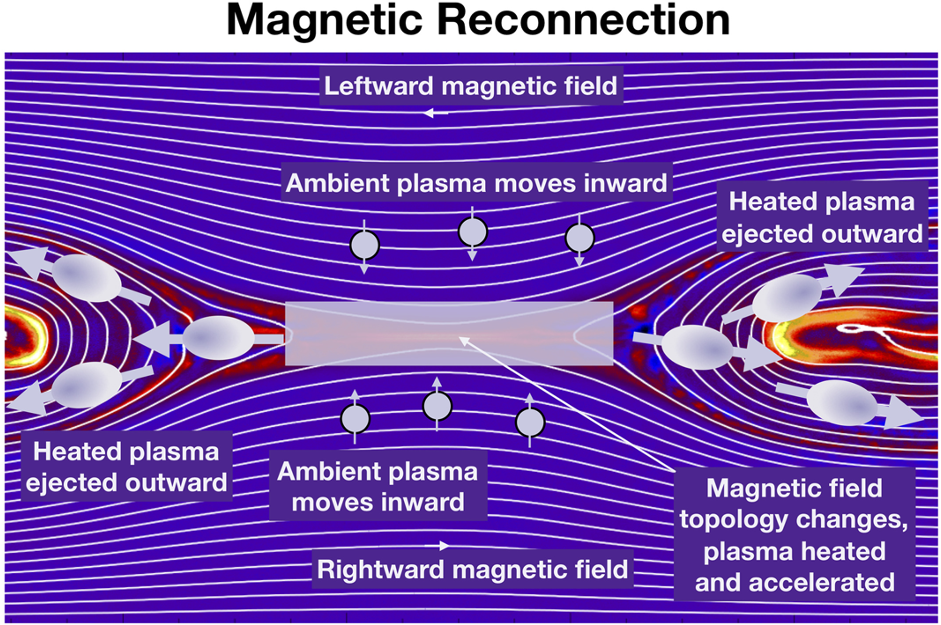
\includegraphics[width=0.8\textwidth]{images1/magnetic-reconnection-cartoon.png}
    \caption{Schematic of magnetic reconnection adapted from \protect\citeA{Hesse2020MagneticFuture} showing the different regions surrounding the X-line.}
    \label{fig:chp1-reconnection-cartoon}
\end{figure}

Figure \ref{fig:chp1-reconnection-cartoon} shows a schematic where two regions with anti-parallel magnetic fields merge and reconnect. Magnetic field lines diffuse towards the center of the region, called the `X-line', via the inflow region and are expelled at large velocities away from the X-line in the outflow regions. Various theories have been put forward to explain and model the reconnection process, to explain the different rates of reconnection observed in different environments (see for e.g. \citeNP{Yamada2010MagneticReconnection} and references therein). In particular, we will discuss the two-fluid model of reconnection. 

In the two-fluid model, the ions and electrons are presumed to demagnetize, i.e. stop following the magnetic field lines, in different regions near the X-line, where the magnetic field strength is at a minimum. The ions, being heavier, are demagnetized first as they enter the \emph{ion diffusion region} and escape via the outflow, where they are accelerated. The electrons remain magnetized until they reach the \emph{electron diffusion region}. The different motions of the electrons and ions generates a current system that in turn produces the quadrupolar Hall magnetic field. As the electron diffusion region is much smaller than that for the ions, it is much difficult to detect in in-situ measurements and remains an active topic for research. Studying the electron diffusion region is the primary objective of NASA's MMS spacecraft constellation, whose goal is to quantify the contribution of various terms in the generalized Ohm's law (e.g. \citeNP{Vasyliunas1975TheoreticalMerging} and references therein) in breaking the frozen-in flux condition \cite{Burch2016MagnetosphericObjectives}.  

\begin{figure}
    \centering
    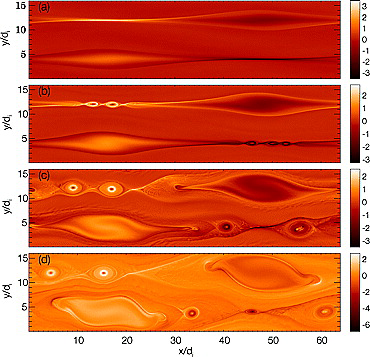
\includegraphics[width=0.8\textwidth]{images1/reconnection-multiplexline-example.png}
    \caption{Example of multiple X-line reconnection adapted from \protect\citeA{Drake2006FormationReconnection}, who have used a particle-in-cell code to simulate anti-parallel magnetic fields. The contours show the out-of-plane component of the current density ($J_z$). Note the progression from steady reconnection to the generation of small magnetic islands at the thin current sheet, which coalesce and evolve to become large magnetic flux ropes or plasmoids.}
    \label{fig:example-multiplexline-reconnection}
\end{figure}

The model shown in Figure \ref{fig:chp1-reconnection-cartoon} represents a situation where magnetic reconnection is occurring in a steady manner. However, particle-in-cell and hybrid simulations of reconnecting fields have shown that this is not necessarily the case. Instead, the thin current sheet near the X-line was found to be unstable to the tearing instability, and breaks into individual closed magnetic loops separated by multiple X-lines \cite{Drake2006ElectronReconnection,Drake2006FormationReconnection}. These magnetic loops, also called flux ropes or O-lines, are created within the ion-diffusion region and are transported away from the X-line through the outflow, where they can coalesce through repeated reconnection and enlarge or dissipate \cite{Markidis2012CollisionlessChain,Wang2016CoalescenceReconnection}. 

The occurrence of magnetic reconnection depends strongly on the angle of magnetic shear between the reconnecting layers, and also on the plasma $\beta$, which is defined as the ratio of thermal pressure ($p$) to the magnetic pressure ($B^2/2\mu_0$) \cite{Swisdak2003DiamagneticMagnetopause,Swisdak2010TheHeliosphere,Phan2010TheObservations}. In particular for asymmetric reconnection, where the two reconnecting layers had a large density gradient, greater differences in plasma $\beta$ across the layers were found to suppress reconnection. This was argued to be the result of fast diamagnetic drifts, which prevented consistent presence of the x-line; which would be advected away with the electron flow, necessitating large magnetic shear angles. On the other hand, reconnection was also seen for small magnetic shear angles during cases when the change in plasma beta across the current sheet was relatively low. \citeA{Swisdak2010TheHeliosphere} proposed a simple relation to gauge the possibility of magnetic reconnection being suppressed in a given setting based on the change in plasma beta $\Delta \beta$ and the magnetic shear angle $\Delta \theta$,

\begin{equation}
    \Delta \beta > \frac{2 L_p}{d_i} \tan\frac{\Delta\theta}{2}
\end{equation}

Where $L_p$ and $d_i$ denote a characteristic pressure-based length scale near the X-line and the ion inertial length, respectively. 

Magnetic reconnection is a fundamental and ubiquitous process in space plasmas and occurs in many different space environments, from the solar corona to the various planetary magnetospheres, to the heliopause. The consequences of magnetic reconnection on the magnetospheres of Earth and Jupiter, and the differences between the two, are discussed in subsequent sections.


\section{Earth's magnetosphere}
A brief description of the processes occurring in the terrestrial magnetosphere is provided in this section to better understand the similarities and differences between it and the Jovian magnetosphere.

\subsection{The solar wind and interplanetary magnetic field}
The solar wind is a stream of particles accompanied by the interplanetary magnetic field (IMF), which flows outward from the sun. It originates from the lower regions of the solar corona, expands and accelerates until it gains a speed roughly between 400 to 600 km/s, by which time it is usually supersonic and super-Alfvenic \cite{Gombosi1998PhysicsEnvironment} i.e. its bulk motion is faster than the local sound and Alfven speeds. It is composed primarily of protons with an average temperature on the order of $10^5$ K and density of $\sim$7 cm$^{-3}$ (at 1 AU = $1.49 \times 10^{8}$ km), though other species and charge states are also present.

It was hypothesized that the radial flow of solar wind plasma distorts the frozen-in interplanetary magnetic field into a spiral configuration with increasing distance from the sun \cite{Parker1958DynamicsFields.,Ness1964SolarField} (see Figure \ref{fig:parker-spiral}). This may be a reasonable assumption during quiet intervals, but the solar wind and IMF can be highly dynamic, leading to the formation of corotating-interaction-regions (CIRs) and coronal-mass-ejections (CMEs). These can be associated with drastic changes in the solar wind dynamic pressure and orientation of the IMF, which perturb the terrestrial magnetosphere in various ways \cite{Borovsky2006DifferencesStorms,Denton2006GeomagneticWind} e.g. by increasing the strength of the equatorial ring current, creating geomagnetically-induced currents on the planet's surface, and strengthening the terrestrial aurora, etc.

Figure \ref{fig:parker-spiral} shows two interplanetary magnetic field lines which intersect the orbits of Earth and Jupiter at 1 AU and 5.2 AU, respectively. The Parker-spiral IMF at Earth typically possesses comparable radial and azimuthal components (where $\mathbf{r}$ is the Sun-Earth direction, also the direction of solar wind flow). On the other hand, the IMF becomes predominantly azimuthal by the time it reaches Jupiter's orbit. This would translate to a near 90-degree magnetic shear between the IMF and the internal field of the planet at the sub-solar magnetopause, which has important implications on the magnetopause reconnection at Jupiter that will be discussed later.

\begin{figure}
    \centering
    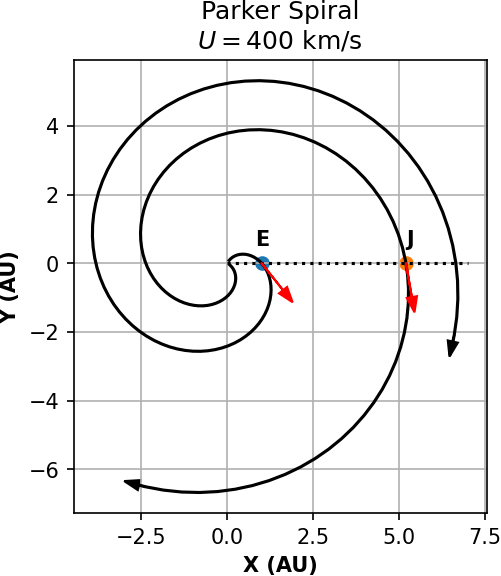
\includegraphics{images1/parker-spiral.png}
    \caption{Interplanetary magnetic field lines showing the Parker-spiral in the ecliptic plane. The field lines intersect at the orbits of Earth and Jupiter at 1 AU and 5.2 AU respectively and the tangent to the curve is highlighted via arrows.}
    \label{fig:parker-spiral}
\end{figure}

\begin{figure}
    \centering
    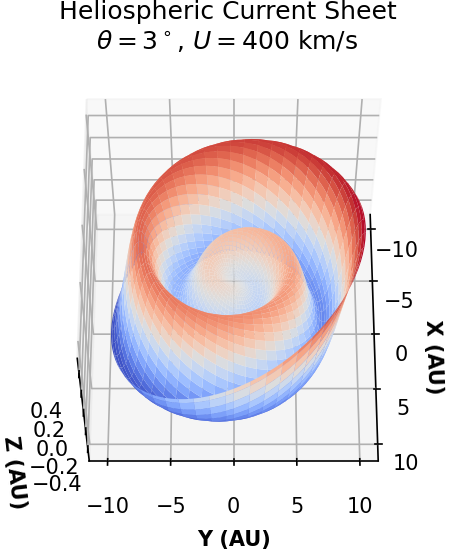
\includegraphics{images1/heliospheric-currentsheet.png}
    \caption{Wavy structure of the heliospheric current sheet assuming a constant 400 km/s solar wind flow and a dipole magnetic field.}
    \label{fig:heliospheric-current-sheet}
\end{figure}

Also associated with the radial outflow of the solar wind is the heliospheric current sheet. Since the solar magnetic axis is not aligned with its spin axis, the heliospheric current sheet undulates about a mean position at the Equator (Figure \ref{fig:heliospheric-current-sheet}). At Earth, this can be seen in the North-South ($Z$) component of the IMF. Periods when the IMF is southward, and thus oppositely directed to the planetary field at the dayside boundaries of the magnetosphere, are considered to lead to increased geomagnetic activity due to magnetic reconnection \cite{Boudouridis2005EnhancedOrientation}. 

\subsection{Configuration of the terrestrial magnetosphere}
The interaction between the solar wind and interplanetary magnetic field with the internal magnetic field of the Earth forms the magnetosphere. Since the incoming plasma is supersonic and super-Alfvenic, a bow shock is created at the interaction front \cite{Spreiter1966HydromagneticMagnetosphere}. Downstream of the shock lies a region of shocked high-temperature solar wind called the magnetosheath \cite{Lucek2005TheMagnetosheath}. The magnetic field strength in the magnetosheath is larger than in the solar wind, but the field lines are still `open', i.e. they are connected at both ends to the interplanetary magnetic field. Separating the planetary field from the magnetosheath is a discontinuity called the magnetopause \cite{Russell1978InitialObservations,Sonnerup1967MagnetopauseObservations}. The magnetopause is a current-carrying layer that shields the magnetosphere from the external inputs.

On the nightside, the interaction of the tail magnetic field with the solar wind and IMF creates a magnetotail \cite{Hones1984StructureActivity}. Magnetic field lines in the magnetotail are considered to be primarily in the plane of the solar wind flow. Present between oppositely directed magnetic field lines in the northern and southern magnetotail lobes is the magnetospheric tail current sheet, which is surrounded by a region of high-density plasma called the plasmasheet. 

In the inner regions of the magnetosphere are the planet's radiation belts; regions of trapped high-energy particles undergoing repeated bounce motions (\citeNP{Ripoll2020ParticleQuestions} and references therein). In these regions the current sheet is weak or non-existent and the magnetic field is close to being dipolar. Co-located with the radiation belts is the plasmasphere, composed of relatively low-energy particles (ions and electrons) which largely corotate with the Earth \cite{Lemaire1998ThePlasmasphere}.

\subsection{Magnetic reconnection in the terrestrial magnetosphere}
In the context of the terrestrial magnetosphere, magnetic reconnection is usually studied in two regions. The first region is the dayside magnetopause, where high density plasma of the magnetosheath associated with a shocked IMF interacts with the relatively low density plasma of the magnetosphere, associated with stronger magnetic fields. Magnetic reconnection has been observed to occur at all orientations of the IMF (clock angle), but is most prominent when the IMF is pointing southward \cite{Swisdak2003DiamagneticMagnetopause}, as in this situation the magnetic shear between it and the northward pointing magnetospheric field (at the magnetopause) is maximized. In such a case, IMF field lines in the solar wind reconnect with `closed' field lines of the magnetosphere, and produce newly opened field lines which are transported away from the reconnection site by the reconnection outflow.

The second region where reconnection is studied widely is the terrestrial magnetotail (e.g. \citeNP{Nakamura2006DynamicsReconnection}). Magnetic field lines in the northern and southern magnetotail lobes which are separated by the magnetotail current sheet are often oppositely directed with respect to each other. Two such open field lines in the magnetotail may spontaneously reconnect and convert into a single closed field line. More often, magnetic reconnection is observed to occur near the planet, where field lines may still be closed, and is preceded by a thinning of the magnetotail current sheet, which results in an explosive reconnection event called a \emph{substorm}. 

Magnetic reconnection in both regions rarely occurs in a steady manner, but instead creates loop-like magnetic structures as seen in Figure \ref{fig:example-multiplexline-reconnection}. At the dayside magnetopause, these structures are referred to as flux-transfer events or FTEs. In the nightside magnetotail, they are referred to as plasmoids or flux ropes, depending on their internal properties. 

\subsection{Ionosphere}
Neutral species in Earth's upper atmosphere can be ionized through photo-ionization and electron impact ionization, and the relatively low-densities at higher altitudes lead to longer collision time scales which supports a persistent region of charged particles called the ionosphere \cite{Schunk2009Ionospheres}. The conducting ionosphere is intricately connected with the magnetosphere.

Ionospheric plasma at mid- to low-latitudes corotates with the planet due to collisions with the corotating thermospheric neutrals. The magnetic field lines associated with these regions are connected at both ends with the planet (i.e. they are \emph{closed}) and have an equatorial footprint in the magnetosphere at a distance of a few Earth radii. Since the field lines in ideal MHD can be considered to possess the same electrostatic potential ($\Phi$), the corotation velocity of the ionospheric plasma is transmitted to the associated magnetic flux tube in the magnetosphere. This creates a corotating region of low-energy plasma called the plasmasphere. This is consistent with the picture that the plasmasphere is a result of $\mathbf{E}\times\mathbf{B}$ drift, where $\mathbf{E}=-\nabla \Phi$ can be considered to be the corotation electric field. Thus, the ionosphere plays a crucial role in maintaining the corotation of plasma at Earth. 

At higher latitudes, magnetic field lines are typically open, i.e. they are connected at one end with the interplanetary magnetic field. In such a case, the ionosphere plays a more responsive role to changes in the solar wind and distant magnetosphere (discussed in the next section). Field aligned currents from the magnetosphere close through perpendicular (to $\mathbf{B}$) currents in the ionosphere. The precipitation of charged particles also modifies the conductivity in the ionosphere \cite{Schunk2009Ionospheres}. 

\subsection{Magnetosphere-ionosphere coupling at Earth}

\begin{figure}
    \centering
    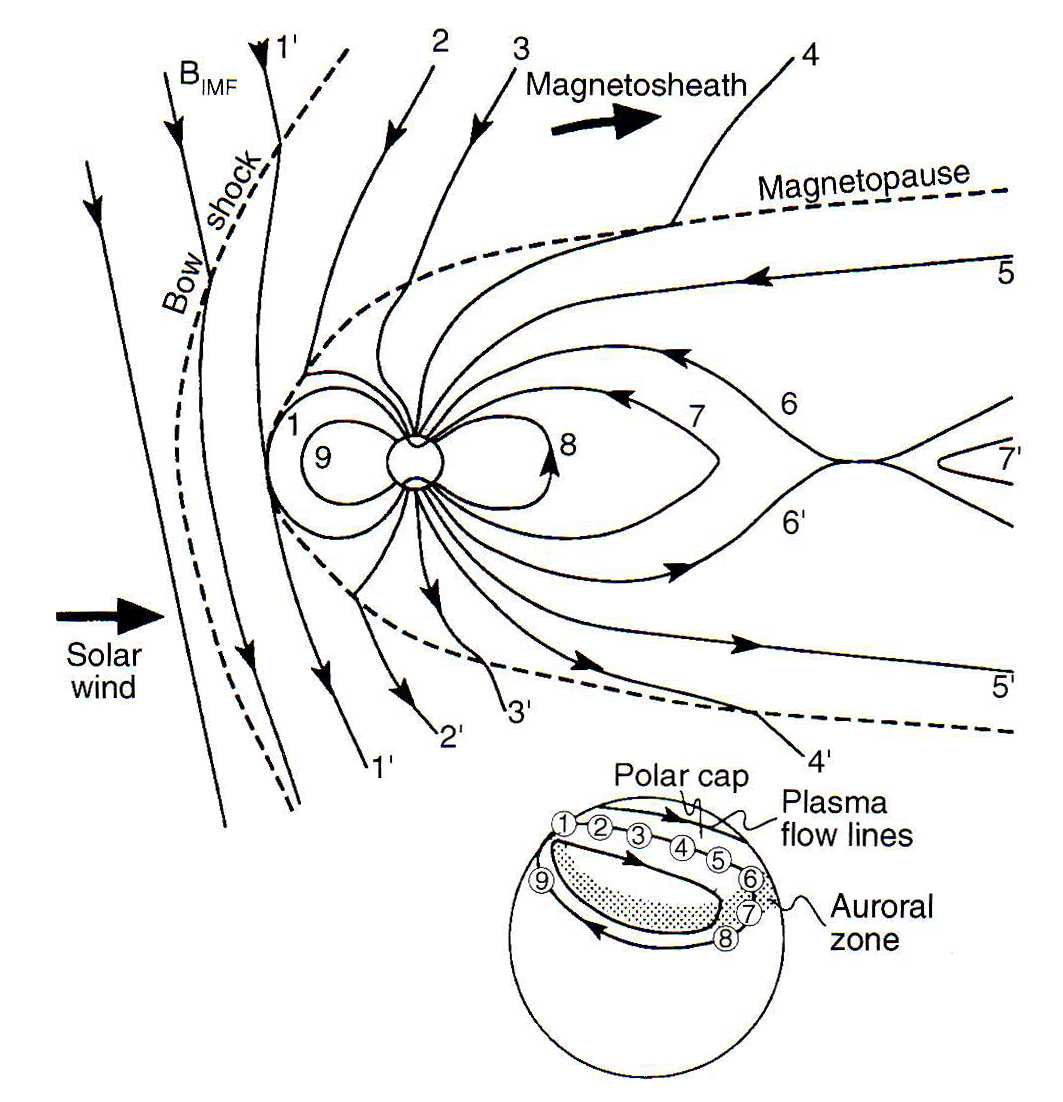
\includegraphics[width=0.9\textwidth]{images1/dungey-cycle.png}
    \caption{Schematic adapted from \protect\citeA{Hughes2019TheReconnection} showing the different stages of the Dungey cycle in the terrestrial magnetosphere and the corresponding convection pattern in the ionosphere.}
    \label{fig:dungey-cycle}
\end{figure}

The magnetosphere and ionosphere are intricately coupled at all latitudes. In the case of anti-parallel IMF, magnetic reconnection on the dayside magnetopause creates open field lines, which convect along with the solar wind. At the same time, one end of the field lines is connected to the polar regions of the planet. Eventually, after reaching the magnetotail, these magnetic field lines are transported into the magnetotail lobes and reconnect. The newly closed magnetic flux returns to the dayside. This cycle of opening and closing of magnetic flux through magnetic reconnection is called the Dungey cycle and an illustration of this process is shown in Figure \ref{fig:dungey-cycle}.

Effects of the Dungey cycle can be seen in the convection patterns of the high-latitude ionosphere (Figure \ref{fig:dungey-cycle}, inset). In the anti-parallel IMF case, ionospheric plasma convects from the dayside to the nightside across the polar cap. After flux closure on the nightside, plasma returns to the dayside via flux tubes located at lower latitudes, on the dawn and dusk side of the magnetosphere; creating a two-cell convection pattern in the ionosphere. This overall convection of the magnetosphere and ionospheric plasma directly determines the location of upward field-aligned currents in the ionosphere, and hence the location of the discrete terrestrial aurora. 

In this way, the solar wind and interplanetary magnetic field directly influence convection in the terrestrial magnetosphere. Different IMF orientations and solar wind density and velocity change the convection patterns in the terrestrial magnetosphere and determine the size of the polar region of open flux,  also referred to as the \emph{polar cap} \cite{Heelis1984TheConvection,Milan2008ResponseOnset}. 

\section{Jupiter's magnetosphere}

Jupiter is a strongly magnetized planet, and the interaction of its planetary magnetic field with the solar wind and IMF creates its magnetosphere \cite{Krupp2004DynamicsMagnetosphere}. Much like at Earth, Jupiter's magnetosphere also consists of a bow-shock, magnetopause and magnetotail because of the supersonic and super-Alfvenic solar wind. However, there are crucial differences due to its large size, strong magnetic field and internal processes associated with its natural satellites. Some key differences between the two magnetospheres are highlighted in Table \ref{tab:earth-jupiter-scales}. Firstly, Jupiter's magnetosphere is much larger than that of the Earth in terms of the planets' respective radii. This is in part due to the strong magnetic field of Jupiter, along with the presence of energetic particles in the magnetosphere, which have a substantial contribution to the total pressure of the magnetospheric plasma \cite{Bagenal2011b}. Note that plasma $\beta$, which is defined as the ratio of thermal pressure $p$ to the magnetic pressure ($B^2/2\mu_0$) is less than 1 for the plasma in most regions of the Earth's magnetosphere, but is between 10 to 100 for plasma in the Jovian magnetosphere.

\begin{table}
    \centering
    \begin{tabular}{p{0.5\linewidth}|c|c}
        &\textbf{Earth}  &\textbf{Jupiter}\\
    \hline
    Equatorial Radius (km) &6378    &71492\\
    Surface field strength (nT)  &$\sim$30000   &$\sim400000$\\
    Internal Source (kg/s)          &5   &250 to $>1000$ kg/s\\
    Rotation Period (hours)         &23.92   &9.92\\
    Dominant species                &H$^+$, O$^+$   &S$^+$, O$^+$, S$^{++}$, H$^+$\\
    Plasma $\beta=p/(B^2/2\mu_0)$   &$<$1 &10 to 100\\
    Magnetopause standoff distance ($R_\text{planet}$)    &8 to 11   &62 to 111\\
    Bow-shock standoff distance ($R_\text{planet}$)   &16 to 22  &77 to 130\\
    Auroral Power (GW)              &20 to 100   &200 to $>$1000\\
    Dipole tilt ($^\circ$)  &$\sim11^\circ$   &$\sim9.6^\circ$\\
    \end{tabular}
    \caption{Comparison of various magnetospheric properties for Earth and Jupiter \protect\cite{Shue1998MagnetopauseConditions,Cairns1996MagneticShock,Khurana2004a, Krupp2004DynamicsMagnetosphere,Clarke2009,Krupp2016ComparisonMagnetospheres,Bagenal2013PlanetaryMagnetospheres}.}
    \label{tab:earth-jupiter-scales}
\end{table}

The Jovian magnetosphere is usually divided into three regions for discussion (1 $R_J$ $=$ 71492 km is the equatorial radius of Jupiter at 1 bar pressure), 

\begin{enumerate}
    \item The inner magnetosphere, containing the Io and Europa plasma tori, which extends up to $r < 15$ $R_J$.
    \item The middle magnetosphere, containing the corotating regions, corotation-enforcement current systems, which ranges from $15 R_J < r < \sim30 R_J$.
    \item The outer magnetosphere, where corotation becomes weak and various dynamics such as magnetic reconnection, Kelvin-Helmholtz instabilities are observed; which lies beyond $r > \sim30 R_J$. 
\end{enumerate}

\subsection{The inner magnetosphere}

A key difference between the gas giant magnetospheres from that of the Earth is the presence of internal sources of plasma associated with their natural satellites \cite{Bolton2015a}. In Jupiter's inner magnetosphere, the largest moons in increasing order of radial distance from the planet are Io (at $5.9$ $R_J$), Europa (at $9.4$ $R_J)$ and Ganymede (at $\sim15$ $R_J$). Out of these, Io and Europa and considered to be un-magnetized, but interact with the surrounding magnetospheric plasma due to the conductive effects of sub-surface magma and saline oceans, respectively. Ganymede is the only known natural satellite in the solar system which possesses a strong internal magnetic field, which interacts with the Jovian magnetic field to create its own magnetosphere \cite{Russell2005InteractionEnvironments,Jia2010MagneticSaturn,Khurana2011EvidenceInterior,Kivelson1996DiscoverySpacecraft,Kivelson2000GalileoEuropa}. 

Out of these satellites, Io and Europa are responsible for contributing substantial mass to the inner magnetosphere of Jupiter. Volcanism at Io creates SO$_2$, which is ionized either via photo-ionization or electron-impact ionization to produce S$^{+}$, S$^{++}$, O$^+$ and H$^+$ (\citeNP{Bagenal2011b} and references therein) etc. Meanwhile, plumes and/or sputtering of the atmosphere at Europa ejects water neutrals into the surroundings, which ionize to produce water group ions e.g. H$^+$, O$^+$. The net contribution of this ionization results in a mass addition of approximately 260-1400 kg/s for Io \cite{Bagenal2011b} and $\sim$50 kg/s for Europa. A similar situation is seen at Saturn, where Enceladus adds $\sim$50 kg/s to its magnetosphere. 

\begin{figure}
    \centering
    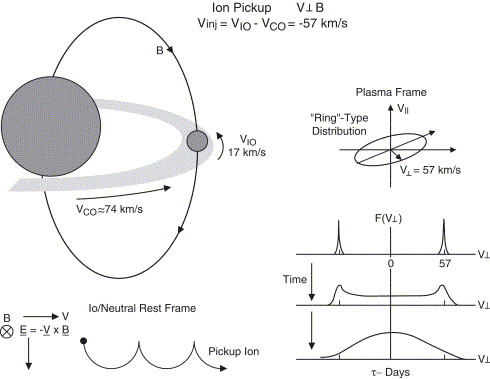
\includegraphics[width=0.8\textwidth]{images1/chp1-io-massloading.jpg}
    \caption{Schematic adapted from \protect\citeA{Russell2005InteractionEnvironments} showing features of mass loading at Io. The magnetospheric plasma is faster than Io's Keplerian velocity. The motional electric field of the corotating plasma ``picks-up'' the newly ionized particles, forming a ring-distribution that relaxes into a stable configuration over many days.}
    \label{fig:io-torus-schematic}
\end{figure}

The newly ionized ions are ``picked-up'' by the surrounding magnetospheric plasma. These ions, which presumably still possess the Keplerian velocity of the neutrals ($\sim$17 km/s at Io's orbit), perceive the motional electric field ($\mathbf{E} = -\mathbf{u} \times \mathbf{B}$) due to the faster magnetospheric flow ($u=\sim74$ km/s) and undergo the $\mathbf{E} \times \mathbf{B}$ drift \cite{Russell2005InteractionEnvironments}. Ion pickup increases particle velocity in the direction perpendicular to the magnetic field, increasing anisotropy in the particle distribution. 

The magnetospheric plasma in the inner magnetosphere co-rotates with the planet. Corotation at these distances is facilitated through ion-neutral collisions in the Jovian ionosphere, which prevents a velocity gradient from forming between the thermosphere and ionosphere; similar to the plasmasphere at Earth. The ionosphere then transmits the velocity to all regions in the magnetosphere with which it is connected via magnetic field lines. The corotation process in the inner magnetosphere does not require the presence of large-scale field aligned currents as in the case of the middle and outer magnetosphere \cite{Vasyliunas1983a}, which we will discuss in the next section.

Also present in inner magnetosphere are trapped energetic particles comprising of Jupiter's radiation belts, which lie outside the scope of the present study. 

\subsection{The middle magnetosphere}

\begin{figure}
    \centering
    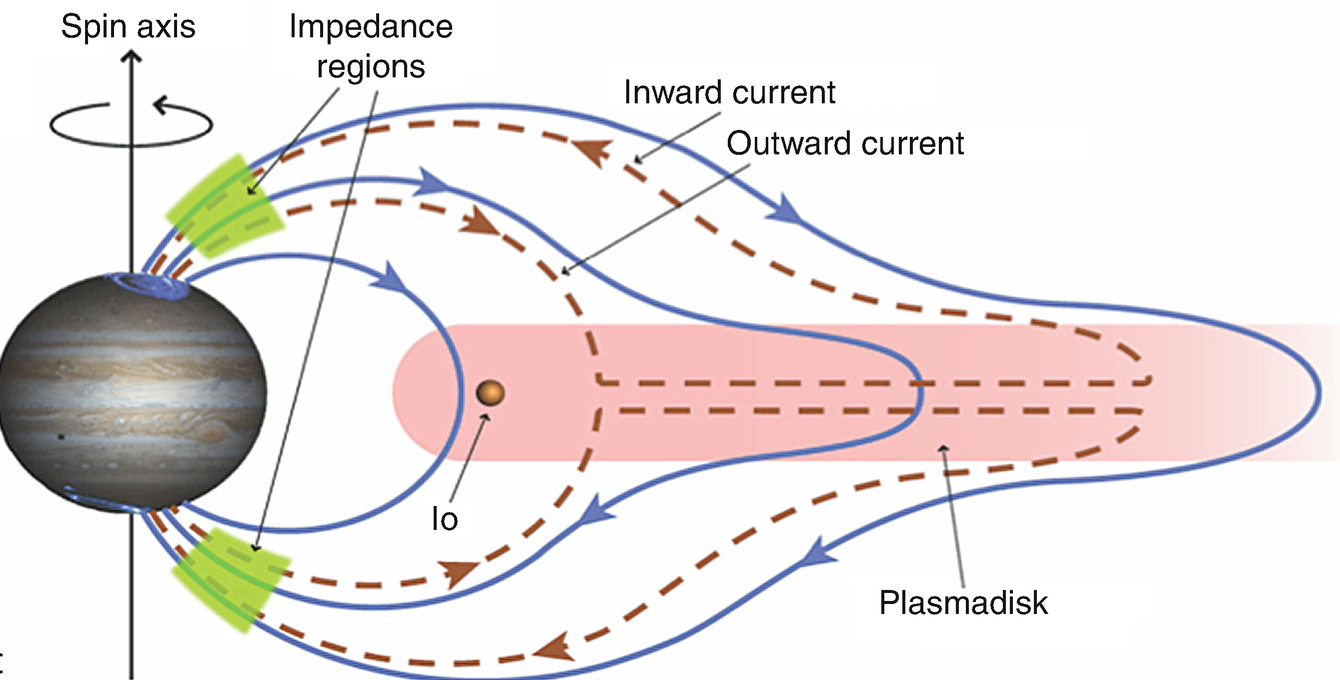
\includegraphics[width=0.9\textwidth]{images1/corotation-schematic.png}
    \caption{Figure adapted from \protect\citeA{Bagenal2013PlanetaryMagnetospheres} showing the extended magnetic field lines in the middle magnetosphere and the the radial currents corresponding to the out-of-plane bend back of the magnetic field. The radial corotation enforcement currents are presumed to be closed through the ionosphere.}
    \label{fig:corotation-schematic}
\end{figure}

The plasma created in the inner magnetosphere of Jupiter is believed to be lost through a series of instabilities. The large density in the inner magnetosphere leads to a decrease in flux tube content with radial distance, which, in the presence of the centrifugal force, creates regions unstable to the interchange instability. Observations by in situ spacecraft have detected plasma and magnetic signatures containing pockets of high magnetic field strength or energetic plasma which is lower in density, within regions of lower energy high-density plasma \cite{Thorne1997GalileoTorus,Kivelson1997IntermittentInterchange}. 

It is believed that as Iogenic plasma moves from the inner magnetosphere to further distances, angular momentum conservation results in the loss of some of its azimuthal velocity \cite{Cowley2001a,Hill2001,Southwood2001a}, also referred to as `breakdown of corotation'. The slowing down of magnetospheric plasma creates a ``bend-back'' of the frozen-in magnetic field lines in the equatorial plane, i.e. the equatorial portions of the magnetic field line begin to lag the regions located at higher-latitudes. The bending of these field lines, or more accurately, the production of magnetic curvature, creates radial currents in the equatorial region to counter the deceleration. The radial currents, together with the predominantly southward magnetic field, create a $\mathbf{J}\times\mathbf{B}$ force in the azimuthal direction, thereby enforcing corotation. These ``corotation-enforcement'' currents are closed via field-aligned currents and perpendicular currents in the Jovian ionosphere. The ionospheric location corresponding to the outward currents (and hence, precipitating electrons) is considered to be the location of the main oval of the Jovian ultraviolet aurora. Figure \ref{fig:corotation-schematic} shows a diagram of the magnetodisc configuration and the expected path of the corotation-enforcement current system.

The centrifugal force in Jupiter's magnetosphere also extends the magnetic field in the radial direction, leading to the formation of an equatorial current sheet at all longitudes, which creates a `magnetodisc' configuration. Evidence for this process has been provided by in-situ spacecraft such as Galileo and Juno, which observed that field lines located at large distances departed greatly from the dipole expectation. 

\subsection{The outer magnetosphere}

\begin{figure}
    \centering
    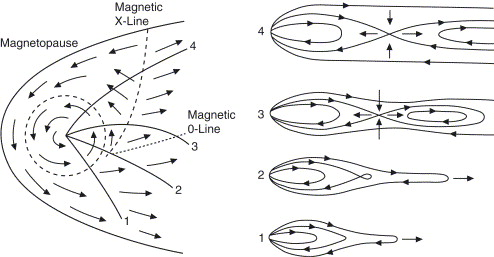
\includegraphics[width=0.8\textwidth]{images1/chp1-vasyliunas-cycle.jpg}
    \caption{Schematic adapted from \protect\citeA{Vasyliunas1983a} and \protect\citeA{Russell2005InteractionEnvironments} showing how a plasmoid is released in the Jovian magnetotail. The image on the left shows the expected flow directions in the equatorial plane, while the different rows on the right correspond to different times during the evolution of a plasmoid.}
    \label{fig:vasyliunas-cycle}
\end{figure}

The mass added by Io and Europa thus corotates with the planet in the inner and middle magnetosphere, and in the process further stresses the magnetic field configuration. It is believed that eventually the stretching of magnetic field lines at large radial distances on the nightside thins the equatorial current sheet to an extent that allows magnetic reconnection to take place in the magnetotail, between two anti-parallel regions of the same field line. 

Magnetic reconnection detaches a loop-like magnetic structures, called a plasmoid, which is disconnected from the other closed field lines and subsequently travels tail-ward to escape the magnetosphere. The newly reconnected closed field line, now devoid of heavy mass, returns to the planet and continues to corotate and re-loaded with mass from the inner magnetosphere. This cycle of mass loss through internal magnetic reconnection is called the ``Vasyliunas'' cycle \cite{Vasyliunas1983a}. The Vasyliunas cycle is considered to be a crucial process that facilitates the loss of Iogenic plasma from the magnetosphere to the external solar wind. Figure \ref{fig:vasyliunas-cycle} shows an illustration of this process in the equatorial and meridional plane. 

Reconnection in Jupiter's magnetosphere occurs differently from the Dungey-cycle reconnection seen in the terrestrial magnetosphere, where open field lines in the magnetotail reconnect and produce a closed field line. At Jupiter, Vasyliunas cycle reconnection is believed to occur spontaneously due to the thinning of the magnetotail current sheet, with no input from the external solar wind and IMF.  

In situ observations have largely confirmed that magnetic reconnection occurs in the Jovian magnetotail, either using magnetic field observations to identify rotations in the north-south component of the magnetic field \cite{Vogt2010a,Vogt2014}, or by detecting bursts of energetic particles with a preference for travel in the radial direction \cite{Woch2002a,Kronberg2008MassParameters, Kronberg2007AMagnetosphere}. However, single-spacecraft observations do not provide information about the global context, and it is unclear whether these reconnection products result from Dungey or Vasyliunas cycle reconnection. 

The relative influence of the solar wind and IMF on reconnection associated dynamics in the Jovian magnetosphere remains an open question. Some authors have argued that Jupiter's magnetosphere is largely closed, and magnetic reconnection on the dayside, if it did occur, could not lead to a persistent polar cap due to the large distances and long timescales involved \cite{McComas2007}. Others have disagreed \cite{Cowley2008}, arguing that both Dungey and Vasyliunas cycle reconnection occur in the Jovian magnetotail, perhaps at different locations, on the dawn-side magnetotail and in the near-midnight region, respectively \cite{Cowley2003a}. 


\section{Jupiter's UV aurora}

\begin{figure}
    \centering
    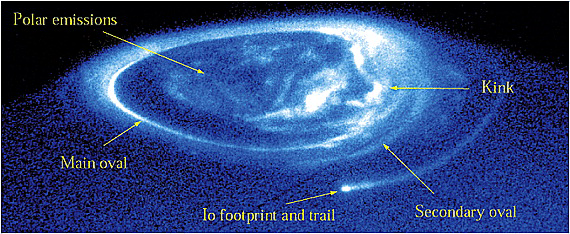
\includegraphics[width=0.9\textwidth]{images1/jupiter-uv-aurora-1.png}
    \caption{Hubble Space Telescope image of the Jovian UV aurora in the northern hemisphere adapted from \protect\citeA{Grodent2003JupitersHST-STIS}, showing its different components. Dawn is roughly to the left of the image, while dusk is toward the right.}
    \label{fig:jupiter-uv-aurora}
\end{figure}

Jupiter produces bright aurora in the ultraviolet spectrum in the polar regions of the planet with typical total power in the range of $10^{12}$ W. The aurora are produced due to electrons of magnetospheric origin precipitating into the ionosphere and causing excitation of H$_2$ or H, which releases photons in the particular spectral range \cite{Grodent2015}. Figure \ref{fig:jupiter-uv-aurora} shows an image from the Hubble Space Telescope of UV auroral emissions from the northern hemisphere of Jupiter.

The Jovian UV aurora is divided into three components for discussion (and highlighted in Figure 
\ref{fig:jupiter-uv-aurora}, with near equal intensities

\begin{enumerate}
    \item The main emission, which maps to regions in the middle magnetosphere. The main auroral oval is present at all longitudes and is thought to be related to the corotation-enforcement current system. It corresponds to the ionospheric location where outward field-aligned currents are expected. Observations have shown that the main oval is thinner at dawn than at dusk, and is weakest in the pre-noon sector. 
    \item The polar aurorae, which occur pole-ward of the main oval and map to regions in the distant magnetosphere or solar wind. The polar aurorae are highly variable and show many repeating features such as `arcs', `swirls' and `filaments'. Their origin cannot be determined without a clear understanding of the magnetic connectivity of the polar regions, and whether they correspond to closed or open field lines.
    \item The equatorward emissions, which map to regions in the inner magnetosphere and are located equatorward of the main emission. These emissions may be a result of wave particle interactions, and could be the equivalent of `diffuse' aurora. They have also been attributed to processes in the inner magnetosphere, such as the interchange instability.
\end{enumerate}

Another set of features seen in the UV aurora are the footprints of Jupiter's natural satellites - Io, Europa, Ganymede and Callisto. These features are related to the satellites' electromagnetic interaction with the Jovian magnetospheric plasma, and are outside the scope of the present work. 

Observations made by the Cassini, HST and Juno spacecraft have hinted that the intensity of the main oval (and the overall aurora) varies according to solar wind dynamic pressure \cite{Nichols2007a,Nichols2017a}, however this is not universally accepted, as most of the time there is no spacecraft to monitor the solar wind conditions upstream of Jupiter. Furthermore, by analyzing simultaneous in situ measurements made by Juno and remote observations by Hisaki spacecraft \cite{Kita2016} find that the auroral response is delayed by almost one Jovian rotation period. On the other hand, both Cassini and Juno had opportunities for simultaneous measurements of the solar wind and the auroral intensity, and find a positive correlation. 

We note that the origin of the Jovian aurora itself remains an active topic of research. Magnetic field signatures corresponding to field-aligned currents have been seen in the Juno magnetometer data near periapsis \cite{Kotsiaros2019BirkelandSpacecraft}, along with inverted-V electron distributions \cite{Mauk2017TheMission}, which originate from discrete acceleration due to large electrostatic potentials. These observations support the theory of corotation-enforcement currents, but \citeA{Bonfond2020SixJupiter} challenge this idea based on recent observations. Field-aligned currents relating to the auroral regions are filamentary and weak \cite{Kotsiaros2019BirkelandSpacecraft}. There is a positive correlation between solar wind dynamic pressure and the Jovian auroral intensity, and bidirectional electron beams have been observed near the auroral regions \cite{Mauk2018DiverseAurora}. 

\section{Objectives of this study}
In this dissertation, we study large-scale dynamics of the Jovian magnetosphere. Specifically, we seek to answer the following questions. 
\begin{enumerate}
    \item How and to what extent does the solar wind influence Jupiter's magnetosphere and currents in the ionosphere?
    \item How does reconnection occur in the Jovian magnetosphere and how are plasmoids released in the magnetotail? To which regions of the ionosphere and aurora do these plasmoids magnetically connect?
    \item How does solar wind dynamic pressure influence the morphology of the magnetotail current sheet?
    \item Where does magnetic reconnection occur in the Jovian magnetotail and are all Jovian plasmoids large and infrequent?
\end{enumerate}

We will attempt to answer questions 1-3 using a global magnetohydrodynamics model, whose details are described in Chapter 2. Chapters 3-5 address each of the questions which are related to large-scale structures in the magnetosphere and can be studied using the global MHD model. In Chapter 6, we analyze data from the Juno spacecraft to form a holistic picture of magnetic reconnection in Jupiter's magnetosphere. 

% \section{Open questions}
% \subsection{Variability of the Jovian UV aurora: Effect of solar wind dynamic pressure?}
% \subsection{Does Dungey-cycle reconnection play an important role?}
% \subsection{How is plasma }

